\chapter{Background}\label{ch:background}

% TODO: Mention that lakehouses (or log structure table formats) are merely a specification and rely on specific implementations to be used, e.g. Spark's implementation of Delta and Iceberg, delta-rs and PyIceberg are all implementations of the spec. In this case, Spark is a query engine, while the other two are libraries that enable interaction with the tables through client APIs. This distinction is especially relevant when comparing the table formats, since it's not fair to compare the performance of a query engine with a client library. 

% TODO: Maybe mention what Parquet is and what the different compression options are, since they are the only relevant config that we will tune in our experiments.

Before we can develop our benchmark, we need to first understand how lakehouses work and which characteristics are relevant to the goal of this thesis. We will look at Iceberg and Delta Lake (Sections \ref{sec:lakehouse-iceberg} and \ref{sec:lakehouse-delta}), which are the two most popular and more mature lakehouse formats based on GitHub stars count and initial release date respectively \cite{thedeltalakeprojectauthorsDeltaLake2026, Iceberg2025}. Moreover, we will look at DuckLake, which brings innovative and relevant features for our research (discussed in Section \ref{sec:lakehouse-ducklake}), despite it still being in version 0.3.

This chapter will also go over the definitions of data stream and throughput, as well as guidelines on performing fair benchmarking.

% We will first go over the different lakehouse technologies included in this thesis: Apache Iceberg, Delta Lake and DuckLake. We will talk about their architectural design, how they handle reads and writes and how they deal with changing data. 

\section{Iceberg}\label{sec:lakehouse-iceberg}
Iceberg was developed in 2017 at Netflix and in 2018 it was released as an open-source project within the Apache Software Foundation\footnote{\url{https://www.apache.org/}}.

\subsection{Architectural design}

\begin{figure}
    \centering
    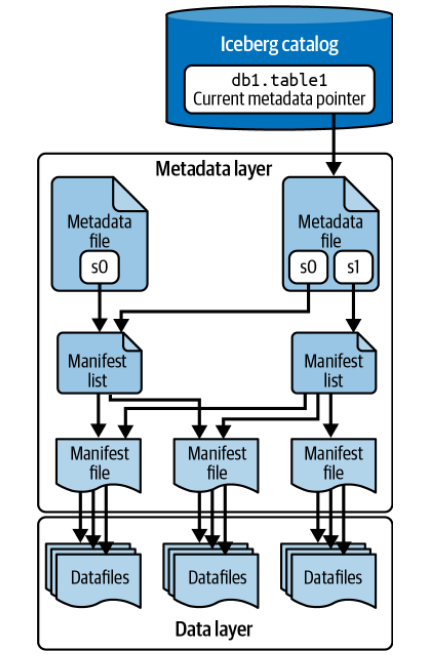
\includegraphics[width=0.45\linewidth]{imgs/iceberg-architecture.png}
    \caption{Architecture of an Iceberg table, as presented in \cite{jasonhughesApacheIcebergDefinitive2024}.}
    \label{fig:iceberg-architecture}
\end{figure}

\subsubsection{Data layer}
 At the base of Iceberg's architecture, there is a data layer, which consists of data files that constitute the Iceberg table. They can be stored in one of three formats: Parquet, ORC\footnote{\url{https://orc.apache.org/}} or Avro\footnote{\url{https://avro.apache.org/}}, with Parquet being the most common due to its widespread adoption and performance gains \cite{jasonhughesApacheIcebergDefinitive2024}.

% The delete files use the same file format as data files, but, as the name suggests, they are a exclusively used for tracking rows that have been deleted from the Iceberg table. There are three different types of delete files in Iceberg, namely:

% \begin{itemize}
%     \item \textbf{Equality delete files}: These files track specific column values that match one or more rows to be deleted from a table \cite{jasonhughesApacheIcebergDefinitive2024}. For instance, if a table contains users' actions on a website, one could delete all actions associated with a user by creating an equality delete file that references that user's id.
    
%     \item \textbf{Positional delete files}: These files keep track of rows to be deleted by storing the path to a data file and the row numbers in that file \cite{jasonhughesApacheIcebergDefinitive2024}. Positional delete files have been deprecated in Iceberg table spec V3 in favor of deletion vectors \cite{apacheicebergIcebergTableSpec}.
    
%     \item \textbf{Deletion vectors}: Introduced in Iceberg table spec V3, deletion vectors replace positional delete files by keeping track of deleted rows of a data file in a bitmap \cite{apacheicebergIcebergTableSpec}. Each vector is associated with one data file, where each bit of the bitmap has the same position as its corresponding row in the data file.
% \end{itemize}

\subsubsection{Metadata layer}\label{sec:iceberg-metadata}

Besides the data layer, there is the metadata layer, which keeps track of the data files locations, the version history of the table, as well as its current schema. The files in the metadata layer are:

\begin{itemize}
    \item \textbf{Manifest files}: Stored in Avro format, these files store pointers to multiple data files, as well as metadata about them, such as the minimum and maximum values of a file's columns and the number of records \cite{jasonhughesApacheIcebergDefinitive2024}. The metadata in manifest files is used for filtering data files during read operations, which helps improve read performance \cite{jasonhughesApacheIcebergDefinitive2024}.

    \item \textbf{Manifest lists}: Manifest lists are another set of Avro files that individually point to a collection of manifest files. Together, the manifest files referenced by a manifest list constitute a specific snapshot, i.e. version, of an Iceberg table \cite{jasonhughesApacheIcebergDefinitive2024}.

    \item \textbf{Metadata files}: These are JSON files that contain schema information about the table, as well as the snapshot history and a pointer to the current snapshot of that table \cite{jasonhughesApacheIcebergDefinitive2024}. A new metadata file is created after every update to the table, marking the creation of a new snapshot. Figure \ref{fig:iceberg-architecture} depicts the architecture of an Iceberg table, where the newest metadata file has a pointer to both snapshots "s0" and "s1".
\end{itemize}

\subsubsection{Catalog}
In order to manage Iceberg tables, a catalog server is used. The goal of the catalog is to point to the latest metadata file of a table, as well as ensure that this pointer is updated atomically \cite{IcebergSpecOptimistic, jasonhughesApacheIcebergDefinitive2024}. Consequently, all interactions with an Iceberg table must go through the catalog server. This avoids inconsistencies when clients are concurrently writing to the same table.

Although many technologies can be used as catalog, e.g. AWS Glue\footnote{\url{https://docs.aws.amazon.com/glue/latest/dg/what-is-glue.html}} and Hive Metastore\footnote{\url{https://hive.apache.org/}}, the developers of Iceberg provide a REST API spec \cite{apacheicebergRESTCatalogSpec2025} as an attempt to unify catalog access across different engines and languages. One prominent implementation of the Iceberg REST catalog is Apache Polaris\footnote{\url{https://polaris.apache.org/}}, which uses a PostgreSQL database to store the latest metadata pointer. 

% \subsection{Reading from Iceberg tables}
% Reading data from Iceberg can be broken down into five steps, as described in \cite{jasonhughesApacheIcebergDefinitive2024}:
% \begin{enumerate}
%     \item The query engine retrieves the pointer to the latest metadata file.
    
%     \item The engine then reads the current table schema and partitioning information, as well as the path to the manifest list.

%     \item From the manifest list, the engine reads the path to the manifest files.

%     \item In each manifest file, the engine checks the data files it points to, possibly skipping over data file partitions that are not included in the query. In addition, the query also checks statistics such as min and max values of columns in the data files, so that it can skip individual data files.

%     \item Once the relevant data files have been selected, the query engine then reads them and returns the result
% \end{enumerate}

\subsection{Writing to Iceberg tables}\label{sec:iceberg-writing}
Writing data to an Iceberg table, e.g. via \verb|INSERT|, involves the following steps \cite{jasonhughesApacheIcebergDefinitive2024}:
\begin{enumerate}
    \item First, the engine checks the catalog to get a pointer to the current metadata file, so that it can read the current table schema.

    \item New data file(s) are written using the chosen storage format for the table.

    \item The engine will then write the manifest file(s) that will contain metadata about the new data file(s), as well as a pointer to them.

    \item Next, a new manifest list file is created, which will point to the new manifest file(s). In addition, existing manifest files are added to this new list, which together will correspond to the new snapshot of the table.

    \item The engine writes a new metadata file which contains a pointer to the new snapshot (manifest list), as well as a history of all previous snapshots.

    \item Finally, following the principle of optimistic concurrency \cite{IcebergSpecOptimistic}, the engine will assume the table has not changed since the start of the operation and will try to atomically update the catalog to point to the new metadata file. However, if a concurrent write has created a new snapshot in the meantime, changing the metadata pointer fails and the engine has to retry. Iceberg tries to structure changes in such a way to minimize the cost of retries \cite{apacheicebergReliability}.
\end{enumerate}

\section{Delta Lake}\label{sec:lakehouse-delta}

Delta Lake was introduced in \citeyear{armbrust_delta_2020} by \citeauthor{armbrust_delta_2020} \cite{armbrust_delta_2020}. It was originally developed at Databricks\footnote{\url{https://www.databricks.com/}} and it was open-sourced in 2022 \cite{tathagatadasDelta20Foundation2022}.

\subsection{Architectural design}

\begin{figure}[h!]
    \centering
    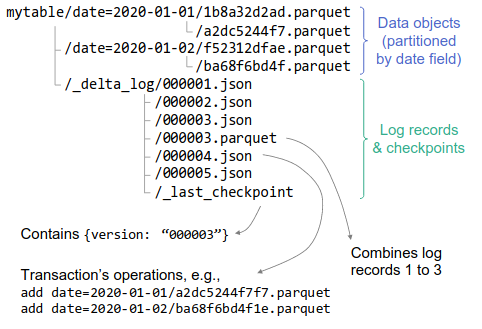
\includegraphics[width=0.6\linewidth]{imgs/delta-architecture.png}
    \caption{The architecture of a Delta Lake table, as presented in \cite{armbrust_delta_2020}.}
    \label{fig:delta-architecture}
\end{figure}

\subsubsection{Data files}

At its core, a Delta table consists of a directory containing data files, which are stored in the Parquet format. As shown if Figure \ref{fig:delta-architecture}, this data can be partitioned to improve efficiency of read queries, but this is beyond the scope of this thesis.

% In addition, Delta stores deletion vectors at the root of a table directory \cite{lee_delta_2025}, which are binary files that keep track of deleted rows of a table. It does so by tracking the offset of a row in the file, its size and the number of rows (cardinality) that has been deleted \cite{lee_delta_2025}.

\subsubsection{Delta log}

The metadata of a Delta table is stored in a subdirectory, called "delta log". This directory contains JSON files, each named in increasing order according to the table version they correspond to, e.g. \verb|00001.json|, \verb|00002.json|, \verb|00003.json|, etc. The log files themselves consist of actions, e.g. \verb|add| and \verb|remove|, that were applied to the data files in order to obtain the respective version \cite{armbrust_delta_2020}.

Furthermore, Delta also keeps track of so-called "checkpoint" files. These are Parquet files consisting of all the actions in the JSON files up until that point in time. These checkpoint files are created periodically (the default being every 10 transactions), so that Delta can stay performant when reconstructing the current state of a table from the log files \cite{armbrust_delta_2020}. The name of the most recent checkpoint file is stored in a \verb|_last_checkpoint| file, as depicted in Figure \ref{fig:delta-architecture}.

\subsubsection{Catalog}

\begin{figure}
    \centering
    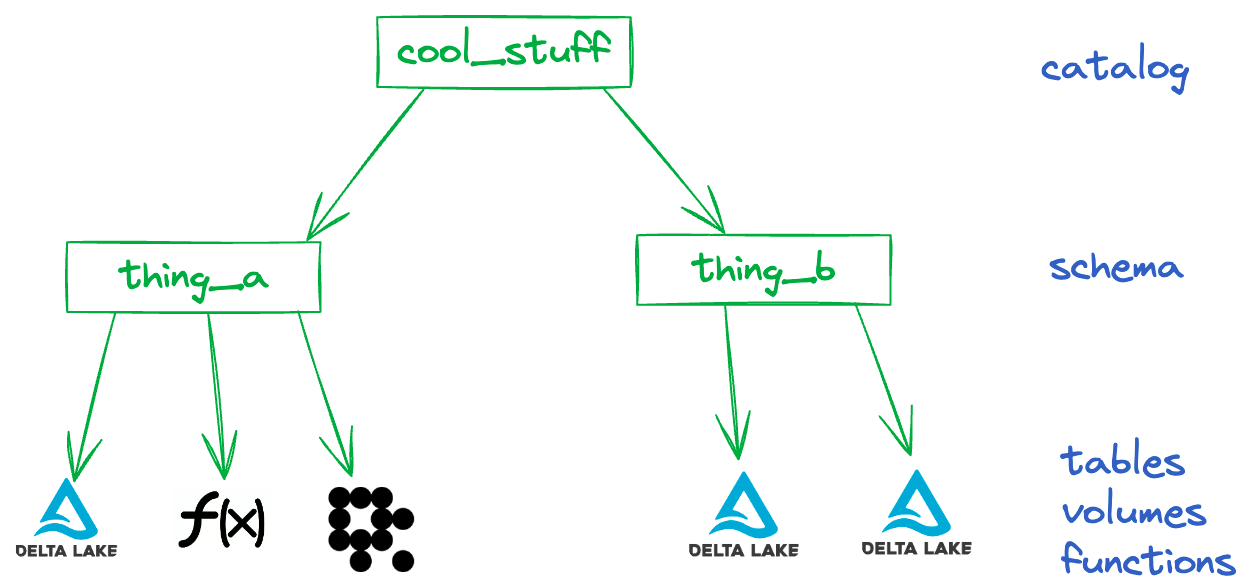
\includegraphics[width=0.8\linewidth]{imgs/unity-catalog.png}
    \caption{Overview of a Unity Catalog, which can be used to manage multiple Delta Lake tables \cite{UnityCatalogStructure2024}.}
    \label{fig:unity-catalog}
\end{figure}

Delta Lake can be connected with a catalog, allowing the management of multiple tables and creating interoperability between other open table formats, such as Iceberg. The most popular catalog used to manage Delta tables is Unity Catalog\footnote{\url{https://www.unitycatalog.io/}}. There are two versions of this catalog: A proprietary version maintained by Databricks and an open-source version. We focus on the latter, since it is freely available. Similar to the Polaris catalog, the Unity Catalog server can be accessed through a REST API and it uses a relational database to store information about the Delta tables that it knows about.

Although a catalog server is not part of the Delta Lake specification, as it is in Iceberg's case, we include it in our research to make sure we perform a fair comparison between the systems we are analyzing (see also Section \ref{sec:benchmarking}).

% \subsection{Reading from Delta tables}
% Below we describe the steps taken by the Delta engine when reading a table \cite{armbrust_delta_2020}:

% \begin{enumerate}
%     \item Delta will first look for the \verb|_last_checkpoint| file. Using the checkpoint file's ID, all subsequent log and checkpoint files are listed.

%     \item Using the listed files, the engine will read them to reconstruct the current state of the table, as well as statistics such as min and max values of columns and partitioning information.

%     \item Based on the table statistics, the engine can ignore files that are irrelevant to the query, which helps improve performance.

%     \item Finally, the relevant data files are queried and the result is returned. 
% \end{enumerate}

\subsection{Writing to Delta tables}
The process of writing data to a Delta table can be broken down into the following steps \cite{armbrust_delta_2020}:

\begin{enumerate}
    \item Delta will first look for the \verb|_last_checkpoint| file. Using the checkpoint file's ID, all subsequent log and checkpoint files are listed.

    \item Using the listed files, the engine will read them to reconstruct the current state of the table, as well as statistics such as min and max values of columns and partitioning information.

    \item Once all those files have been read, new data objects are written (possibly in parallel) to the underlying file storage.

    \item Then, assuming the latest log file has ID $n$, Delta attempts to create a new log file named $n+1$\verb|.json|. Since there can only be one file corresponding to a specific version of the table, creating the new log file needs to happen atomically. If this step fails due to a concurrent write operation, the transaction can be retried.

    \item (Optional) Depending on the configured interval for writing checkpoints, a new checkpoint file will be created and the \verb|_last_checkpoint| file is updated to reflect that change.
\end{enumerate}

It is important to note that, like in Iceberg (Section \ref{sec:iceberg-writing}), optimistic concurrency control is employed for write operations. However, Delta relies on the underlying object store's mechanism to ensure transaction atomicity \cite{armbrust_delta_2020}. For instance, Azure Blob Store, Google Cloud Storage and Amazon S3 support conditional write operations \cite{SpecifyingConditionalHeaders2025, RequestPreconditions2026, HowPreventObject}, thus ensuring that only one client can create a log file with a specific name.

% So if a new log file ($n+1$\verb|.json| in this case) is created between the start and end of a write operation, that operation fails and needs to retry. Again, as it is the case for Iceberg, there are optimizations in place that allow the engine to retry the operation without having to rewrite all files, depending on the query \cite{armbrust_delta_2020}. In any case, this can lead to overhead when concurrent writes are happening in Delta Lake.

\section{DuckLake}\label{sec:lakehouse-ducklake}
DuckLake is an open table format introduced in 2025 as part of the DuckDB Foundation. Although it is currently an experimental release (as of writing, the current version is 0.3 \cite{guillermosanchezDuckLake03Iceberg2025}), we believe it will be a valuable addition to our research, as its specification proposes a new way of storing metadata and an interesting approach for handling changes to its tables.

\subsection{Architectural design}

\begin{figure}
    \centering
    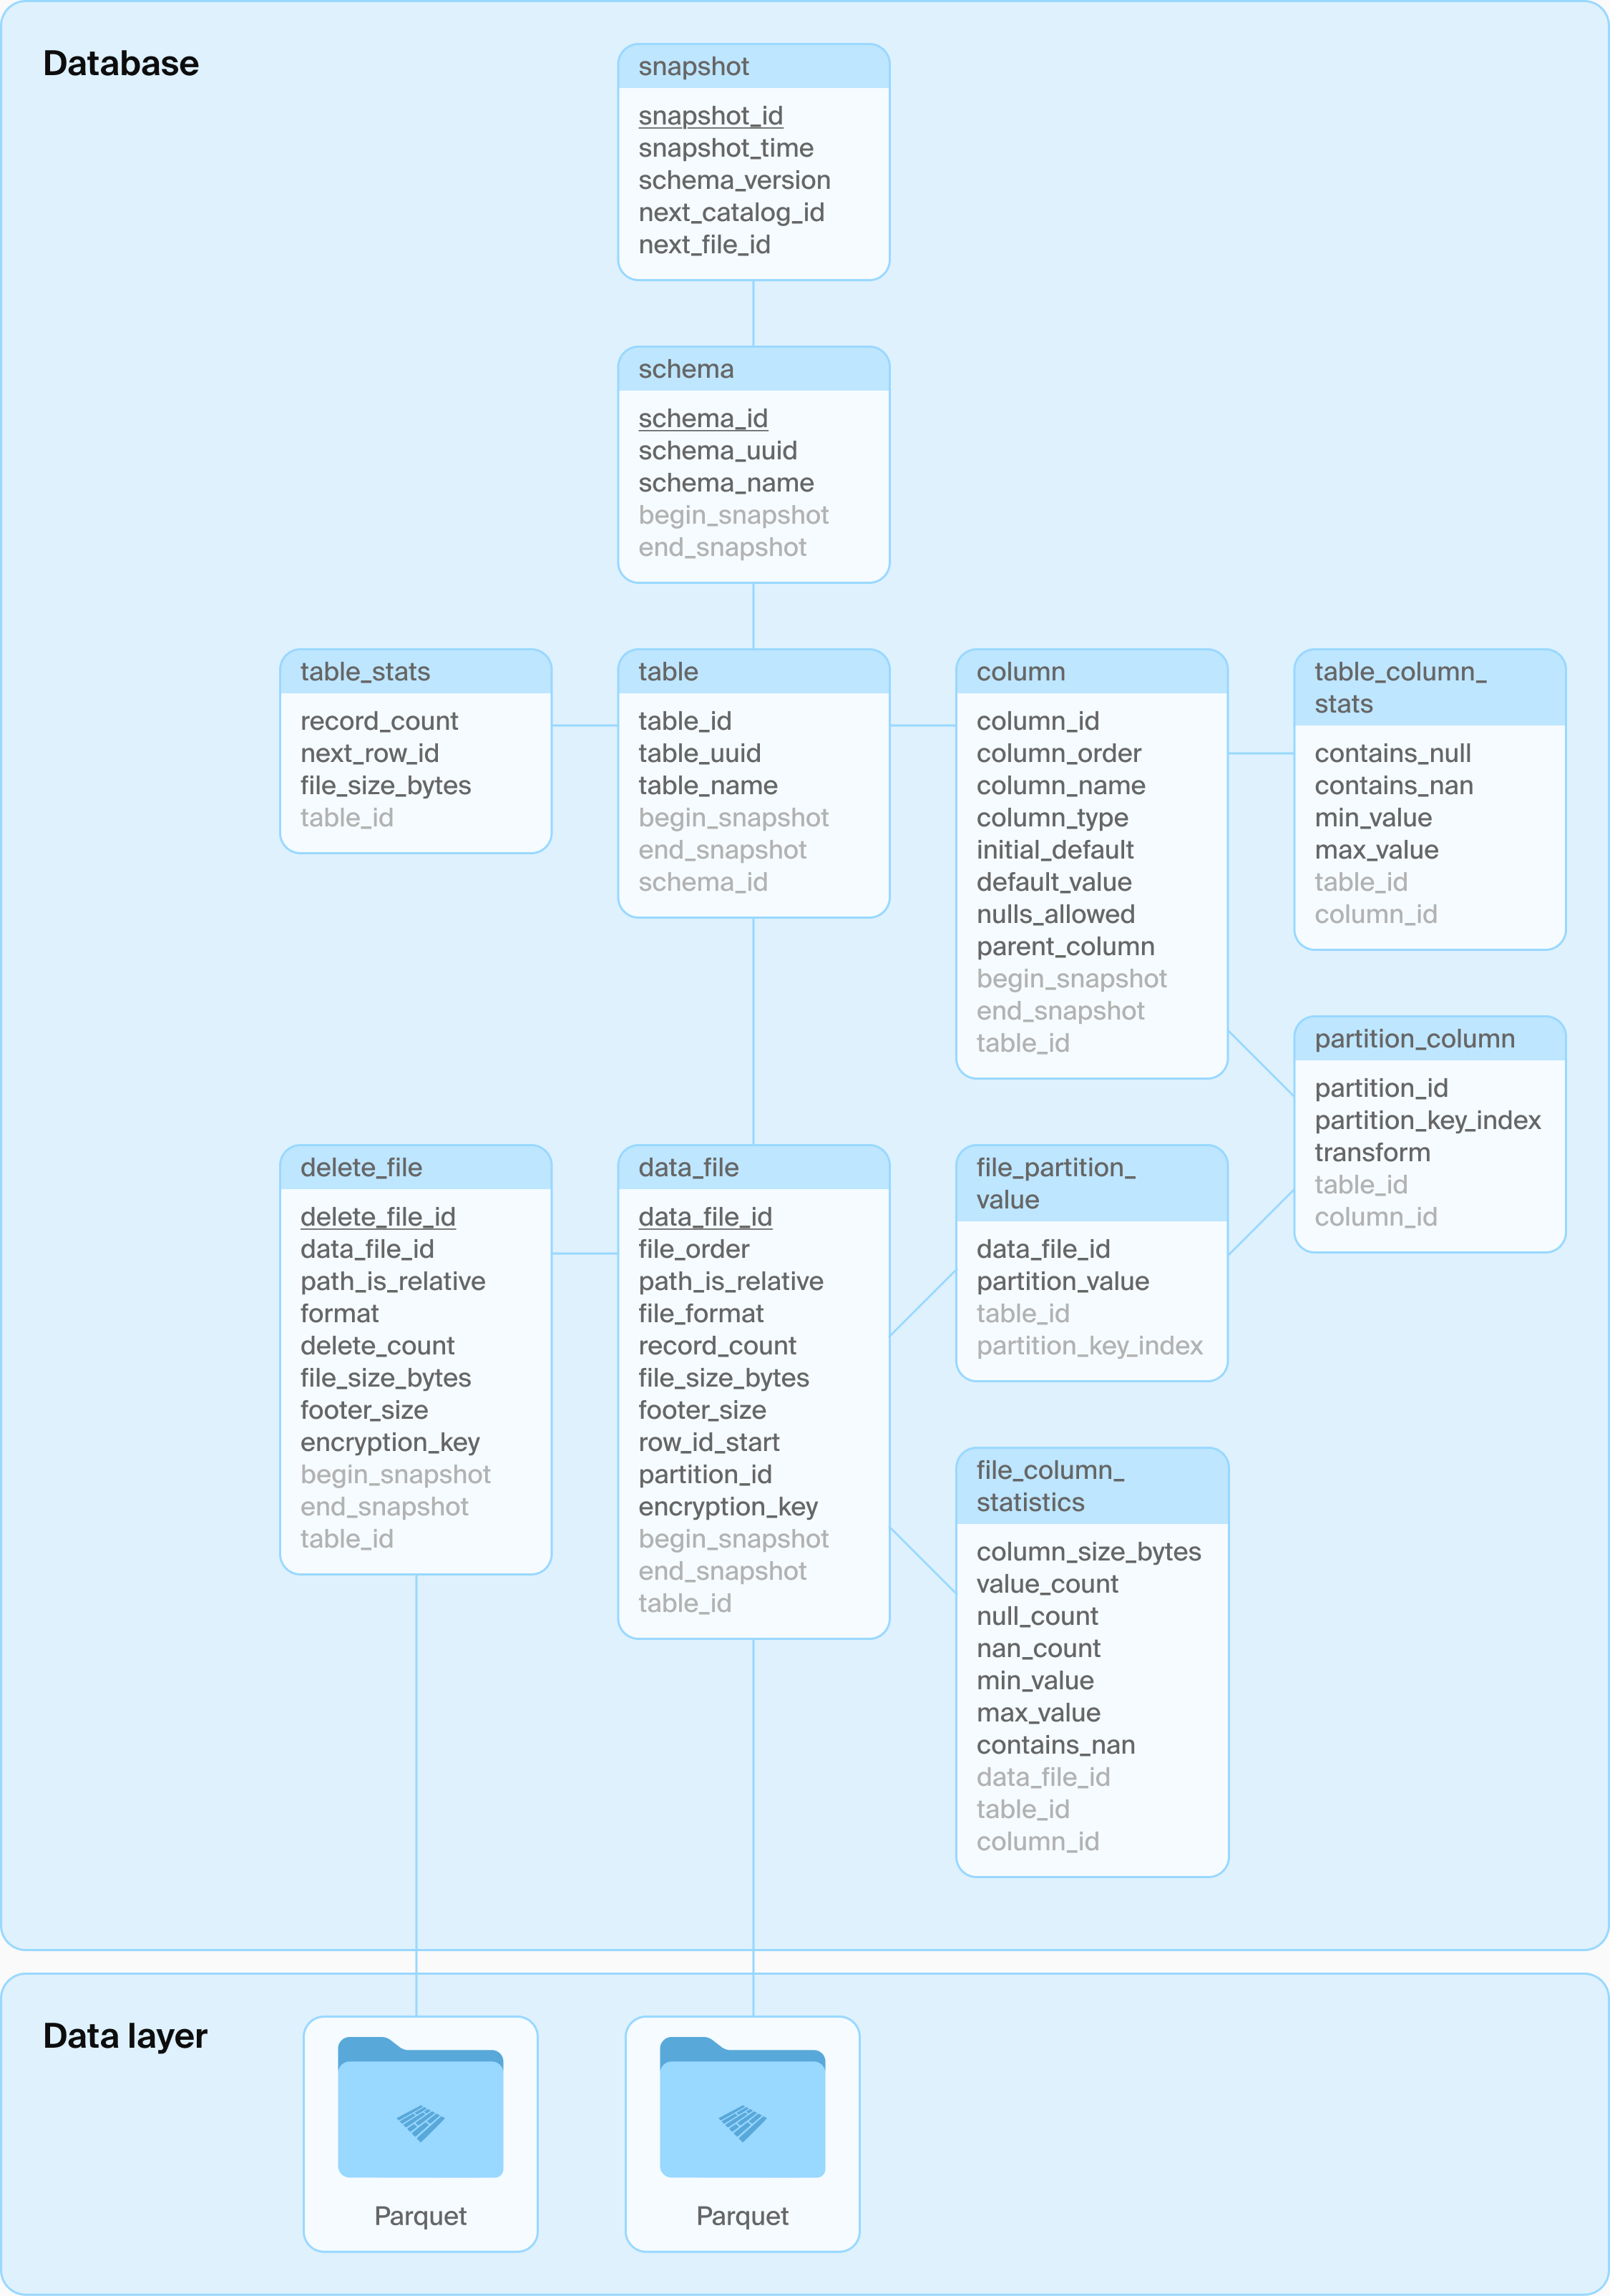
\includegraphics[width=\linewidth]{imgs/ducklake-architecture.png}
    \caption{Architecture of a DuckLake table, as presented in \cite{mark_raasveldt_ducklake_2025}.}
    \label{fig:ducklake-architecture}
\end{figure}

\subsubsection{Data layer}
DuckLake's data layer consists of Parquet data files on the chosen storage system, which make up the table.

\subsubsection{Catalog database}
Similar to Iceberg, DuckLake also includes a catalog in its specification. However, DuckLake's catalog differs from Iceberg's in that it stores all of the table's metadata instead of storing the pointer to the current metadata file. In total, the catalog database contains 22 tables that together keep track of the schema, snapshots, data files, tables, statistics and partitioning information of DuckLake tables \cite{DucklakeDocumentationTables2025}. Currently, DuckLake supports DuckDB\footnote{\url{https://duckdb.org/}}, SQLite\footnote{\url{https://sqlite.org/index.html}}, PostgreSQL and MySQL\footnote{\url{https://www.mysql.com/}} as its catalog database \cite{DucklakeDocumentationChoosing2025}. Figure \ref{fig:ducklake-architecture} shows the most relevant tables stored in the catalog \cite{DucklakeDocumentationTables2025}:

\begin{itemize}
    \item \verb|table|: This is where the DuckLake tables' name, path and schema are stored. In addition, it tracks the snapshot interval in which the table is valid.
    
    \item \verb|table_stats|: This contains metadata about the DuckLake tables, such as the number of records and the total file size of the data files that compose this table.
    
    \item \verb|column|: This table stores the columns that are part of the DuckLake table. The main attributes are the column's name, its type and default value.
    
    \item \verb|table_column_stats|: Similar to \verb|table_stats|, this table contains metadata about each column in a DuckLake table, e.g. min and max values and whether the column has \verb|NULL| values.
    
    \item \verb|partition_column|: Contains partitioning information about columns on which partitioning has been enabled. It also stores the transformation function that is applied to the column to obtain the partition key, if such a function is required. For instance, if a table contains a timestamp column, one can apply a transformation function to that column and use the resulting value as the partitioning key.    
    
    \item \verb|data_file|: This table stores information about the data files, such as the path, format (for now, only Parquet is allowed \cite{DucklakeDocumentationTables2025}), number of records in the file and the size in bytes.

    \item \verb|file_column_stats|: Similar to \verb|table_column_stats|, this table stores column statistics on a file level, e.g. amount of records, min and max values and number of \verb|NULL| values.

    \item \verb|delete_file|: Similar to \verb|data_file|, this table stores the path and format of delete files\footnote{Delete files are used to mark which records have been deleted from a table without actually deleting any files. This is done because Parquet files are immutable and would have to be rewritten every time a record is updated or deleted. By using delete files, deleted records can be reconciled at read time in a process called merge-on-read (MoW) \cite{paras_jain_analyzing_2023}, which is beyond the scope of this thesis.}, but it contains the number of records deleted by the file.

    \item \verb*|snapshot|: This table is used for representing the snapshots, i.e. versions, of the DuckLake instance. Every change to a table will result in a new snapshot with a corresponding timestamp.

    \item \verb|snapshot_changes|: For each snapshot, this table stores a list of changes that were made to the DuckLake instance, e.g. \verb*|CREATE|, \verb*|INSERT|, \verb*|UPDATE|, \verb*|ALTER|.

    \item \verb|schema|: This table stores the different schemas that can be used to separate DuckLake tables into namespaces. The table stores the schema name, its path in the file system, as well as the snapshot interval in which that schema is valid.
\end{itemize}

%\subsection{Reading from DuckLake tables}
%Reading from a DuckLake table goes as follows \cite{DuckLakeDocumentation2025}:
%
%\begin{enumerate}
%    \item DuckLake first reads the latest snapshot number from the \verb|ducklake_snapshot| table.
%
%    \item Then, it reads the valid schemas in the current snapshot from \verb|ducklake_schema|. By default all tables are stored under the \verb|main| schema.
%
%    \item Next, DuckLake lists the tables in the given schema.
%
%    \item For the tables, it lists all the columns to determine the table structure.
%
%    \item Knowing the table structure, DuckLake queries the data files and delete files, so that it can know which rows to display and which ones have been deleted.
%\end{enumerate}

\subsection{Writing to DuckLake}
Writing to DuckLake tables happens in the following steps \cite{mark_raasveldt_ducklake_2025}:

\begin{enumerate}
    \item First, the Parquet files are written to storage, unless data inlining (\ref{sec:ducklake-inlining}) is enabled and the number of inserted rows is lower than the set threshold.

    \item Then, in a single database transaction, the following tables are updated to reflect the new changes: 
    \begin{itemize}
        \item \verb|data_file|
        \item \verb|table_stats|
        \item \verb|table_column_stats|
        \item \verb|file_column_statistics|
        \item \verb|snapshot|
        \item \verb|snapshot_changes|
    \end{itemize}
    DuckLake enforces a primary key constraint on the snapshot id in the \verb|snapshot| table \cite{DuckLakeDocumentationConflict2025}. If two clients try to concurrently create a new snapshot, one of them will fail due to a \verb*|PRIMARY| \verb*|KEY| constraint violation \cite{DuckLakeDocumentationConflict2025}. In that case, DuckLake will try to solve the conflict without having to rewrite the data files. For that, it looks at the \verb|snapshot_changes| table to see what changes were made by the transaction that succeeded. If there are no logical conflicts, e.g. both clients just added new data, the failed client can retry the transaction without having to rewrite the data files \cite{DuckLakeDocumentationConflict2025}.
\end{enumerate}

\subsection{Data inlining}\label{sec:ducklake-inlining}
One feature that sets DuckLake apart from Delta and Iceberg is the so-called "data inlining". This feature allows DuckLake to be configured such that writes that insert fewer rows than a set threshold are stored in the catalog database, rather than written out as Parquet files \cite{DuckLakeDocumentationData2025}. This can increase the performance of DuckLake for frequent, small, updates. The "inlined" data is immediately visible for read operations and it can be flushed out to Parquet files once enough data has been accumulated in the catalog \cite{DuckLakeDocumentationData2025}.

% TODO: Probably remove this section, since we're not doing any updates.
%\section{Data update strategies}
%
%\subsection{Copy-on-write (CoW)}
%This update strategy is supported by both Delta and Iceberg and, as the name suggests, it consists of rewriting the data files when a table is updated or data is deleted to reflect those changes. This results in higher write latency in favor of faster reads \cite{paras_jain_analyzing_2023}.
%
%The main reason CoW exists is because file formats used for data files, e.g. Parquet, are immutable \cite{matthewpowersDeltaLakeVs}, which means that changing a single value in them requires a complete rewrite of the file. In addition, lakehouses make use of snapshots to provide "time traveling" features, which is only possible by storing the older version of data files in the lakehouse storage layer.
%
%\subsection{Merge-on-read (MoR)}
%By using deletion vectors, or other delete file types in the case of Iceberg and DuckLake, (see Sections \ref{sec:lakehouse-iceberg} and \ref{sec:lakehouse-delta}), it is possible to adopt a merge-on-read (MoR) strategy instead of CoW. In this case, no data files are rewritten during updates and deletes, but rather the affected rows are stored in deletion files, usually in binary format, which are then used to filter out the corresponding data from the table during read operations. This strategy favors faster writes, but adds extra overhead when reading a table, since the engine needs to resolve the deleted rows of each table by reading the delete files. 
%
%It is worth mentioning that the table size and the number of updated/deleted rows are of great influence to the effectiveness of delete files and MoR. For instance, if the table consists of only a few data files and the amount of affected rows comprises a high percentage of the table, the time difference between writing a deletion file and rewriting the data files might be negligible, in which case rewriting the table would be preferable (CoW), since there would be no additional overhead when reading the table later. However, if the table is partitioned into multiple data files, changes to rows could lead to rewriting many files, in which case deletion files would be beneficial.
%
%In order to keep lakehouses performant when using MoR, it is recommended to perform regular maintenance operations, which rewrite data files with a high number of deleted rows into fewer, or even a single, data file(s) \cite{DuckLakeDocumentation2025, nickkarpovDeltaLakeDeletion2023, apacheicebergMaintenance}.

% \section{Stream processing}
% Streaming data can be defined as data that is produced by one or more sources continuously and thus, is considered unbounded \cite{tylerakidauStreaming101World2015, fragkoulisSurveyEvolutionStream2024}. As opposed to finite datasets that can be processed in their entirety by methods such as MapReduce \cite{jeffreydeanMapReduceSimplifiedData2004}, streaming datasets usually do not have a "final" data point, so streaming processing engines (SPEs) rely on approaches such as (micro-)batching and windowing to create finite groupings from the unbounded data for processing \cite{tylerakidauStreaming101World2015}. Some use cases where stream processing is commonly applied, include IoT sensor-monitoring, fraud detection, advertisement analytics and processing of logs for web services \cite{yueSurveyStreamProcessing2026}.

% In the following sections, we will lay out the core concepts of streaming data processing that we will be referring to throughout this thesis. 

% \subsection{Event time}
% One of the core concepts of data stream processing is "event time", which refers to the timestamp when a given event was produced by a source \cite{tylerakidauStreaming101World2015, yueSurveyStreamProcessing2026}, e.g. an IoT sensor. Event time is primarily used for windowing events, which we will discuss later on.

% \subsection{Processing time}
% As the name implies, processing time refers to the moment when an event is processed by a streaming system. This is not necessarily equal to the time when an event enters the streaming system, sometimes referred to as "ingestion time" \cite{yueSurveyStreamProcessing2026}, but rather the time when the event is sent for downstream processing \cite{tylerakidauStreaming101World2015}, usually after a fixed time period.

% \subsection{Processing patterns}
% When it comes to actually processing the data, there are different techniques that SPEs apply to process unbounded streams of data in some type of bounded way.

% \subsubsection{(Micro) Batching}
% % Spark operates in this mode by default, with a default interval of 500ms (source: https://docs.databricks.com/aws/en/structured-streaming/triggers)
% The first way of processing streaming data is by grouping incoming data in batches that are processed at fixed time intervals. Since the interval is fixed, micro-batching relies solely on the processing time to create the micro batches. These intervals are usually kept at low values, e.g. Spark\footnote{\url{https://spark.apache.org/docs/latest/streaming/index.html}} uses intervals of 500ms by default \cite{ConfigureStructuredStreaming2023}, so that latency is kept at a low rate.

% \subsubsection{Windowing}
% Windowing is a more flexible technique for processing data streams, as it allows grouping events by both processing and event time \cite{tylerakidauStreaming101World2015}. There are three main types of windowing techniques, namely:

% \paragraph{Fixed windows}
% Also referred to as "tumbling window", this method groups events in non-overlapping fixed-length windows, which are then sent for downstream processing. When creating windows by processing time, this method works essentially the same way as micro-batching.

% \paragraph{Sliding windows}
% These windows also consist of a fixed time length, but the period in which they occur may be different than their length, which results in overlapping windows. In case the step 

% \paragraph{Session windows}

% \subsection{Processing guarantees}

% \subsubsection{At least once}
% \subsubsection{At most once}
% \subsubsection{Exactly once}

% \cite{fragkoulisSurveyEvolutionStream2024}. Although systems can accumulate batches of data to process, a streaming dataset has 

% \citeauthor{fragkoulisSurveyEvolutionStream2024} provide an extensive overview of the core characteristics of streaming systems in \cite{fragkoulisSurveyEvolutionStream2024}

\section{Data streams}\label{sec:data-streams}
A data stream can be defined as data that is produced by one or more sources continuously and thus, is considered unbounded \cite{tylerakidauStreaming101World2015, fragkoulisSurveyEvolutionStream2024}. Examples of data streams are measurements produced by IoT sensors, web server logs and network traffic data. Another key characteristic of stream data is the presence of at least one timestamp, which is assigned when the data point, i.e. event, is produced or processed by a system \cite{fragkoulisSurveyEvolutionStream2024}.

\section{Benchmarking}\label{sec:benchmarking}
When it comes to evaluating systems' performance, it is crucial that the comparison is done fairly to avoid misleading results. In that regard, \citeauthor{raasveldtFairBenchmarkingConsidered2018} \cite{raasveldtFairBenchmarkingConsidered2018} highlight some of common pitfalls when benchmarking database systems. These pitfalls were obtained from a literature review on best practices and recommendations for both benchmarking in general and benchmarking of database management systems (DBMSs). The authors then identified seven\footnote{In the original paper, the authors report "cold" vs "hot" runs and "cold" vs "warm" runs separately \cite{raasveldtFairBenchmarkingConsidered2018} , so they reported eight pitfalls in total. We believe however that they pertain to the same aspect of benchmarking, so we include them all in the same pitfall.} different pitfalls that can occur during DBMS benchmarking, namely:

\begin{enumerate}
	\item \textbf{Reporting non-reproducible results}: In scientific research in general, it is required that results are reproducible, so that they can be independently verified. Benchmarking is no exception to this rule.
	
	\item \textbf{Sub-optimally optimizing systems}: In cases where the authors of a paper are comparing their own system with the state of the art, they might feel tempted to not properly optimize the systems they are comparing with, so that they get favorable results \cite{raasveldtFairBenchmarkingConsidered2018}. In some other cases, failure to properly optimize a system might happen due to lack of familiarity with that system.
	
	\item \textbf{Overly-optimizing a system}: Similarly to the previous pitfall, one might optimize their system to perform really well on a specific benchmark. This can be done by optimizing a system for the specific dataset or workloads present in a benchmark, which are all known prior to execution.
	 
	\item \textbf{Benchmarking code that contains bugs}: Sometimes, performance measurements can be influenced by bugs in the SUTs or in the code performing the benchmark. Bugs can lead to an unfair advantage by skipping a step of the benchmark workload or by only working with a specific dataset \cite{raasveldtFairBenchmarkingConsidered2018}.
	
	 
	\item \textbf{Comparing systems that are fundamentally different}: Benchmark results can only be considered fair if they were obtained from systems that provide the same functionality. Otherwise, one of the systems might be given an unfair advantage by avoiding a set of constraints present in other systems. \citeauthor{raasveldtFairBenchmarkingConsidered2018} \cite{raasveldtFairBenchmarkingConsidered2018} exemplify this by comparing a complete DBMS with an algorithm specialized in one task. The algorithm has an advantage because it takes fewer aspects into account than the DBMS \cite{raasveldtFairBenchmarkingConsidered2018}.
	
	\item \textbf{Ignoring preprocessing time}: When running benchmarks, the SUTs often have to be initialized with the dataset used in benchmark's workload. This initialization can sometimes include preprocessing steps that a system executes to speed up performance of subsequent tasks. The example given in \cite{raasveldtFairBenchmarkingConsidered2018} mentions the creation of database indexes, which if ignored, might favor a system that has efficient, but slow-to-create, indexes.
	
	\item \textbf{Comparing "cold", "warm" and "hot" runs}: The concept of a "cold" run refers to executing a benchmark for the first time on a system for which no data has been cached on the host operating system yet. By contrast, subsequent runs of the benchmark are considered "hot", due to the creation of caches and other optimizations that the underlying operating systems might execute. \citeauthor{raasveldtFairBenchmarkingConsidered2018} \cite{raasveldtFairBenchmarkingConsidered2018} also alert for "warm" runs, which can occur when the SUT is restarted to perform a "cold" run, but caches are still present in the OS memory \cite{raasveldtFairBenchmarkingConsidered2018}.
	
\end{enumerate}

In addition, the authors in \cite{raasveldtFairBenchmarkingConsidered2018} suggest practices on how to prevent these pitfalls from happening. In some cases, such as that of non-reproducible experiments, it can be easily avoided by including a detailed specification of the configuration parameters used, hardware specifications and source code. However, other pitfalls are not so trivial to avoid. For instance, making sure the SUTs are not running sub-optimally can be hard depending on the amount of configuration available for each system. Nonetheless, we will follow the checklist provided in \cite[Appendix~A]{raasveldtFairBenchmarkingConsidered2018} and mention it whenever relevant throughout this thesis. 
% Maybe introduce the paper "Fair Benchmarking Considered Difficult" and mention the concepts we'll be using in our project. Otherwise, maybe remove this section and just talk about benchmarking in related work.
% \cite{petetuckerNEXMarkBenchmarkQueries2008}
